% !TEX TS-program = lualatex
%\documentclass[handout]{beamer}
\documentclass{beamer}
\input{../common/misomva}
\begin{document}
% Topic-specific title slide

\newcommand{\topictitle}{Graph Theory Basics}

\newcommand{\topicsubtitle}{Seven Bridges of Königsberg}
\newcommand{\misoclasstinytitleslide}{Partially based on material by:  Andreas Krause, \\[-1em] Branislav Kveton, Michael Kearns}

\MakeTopicSlide

\begin{frame}
\frametitle{Graph theory refresher}
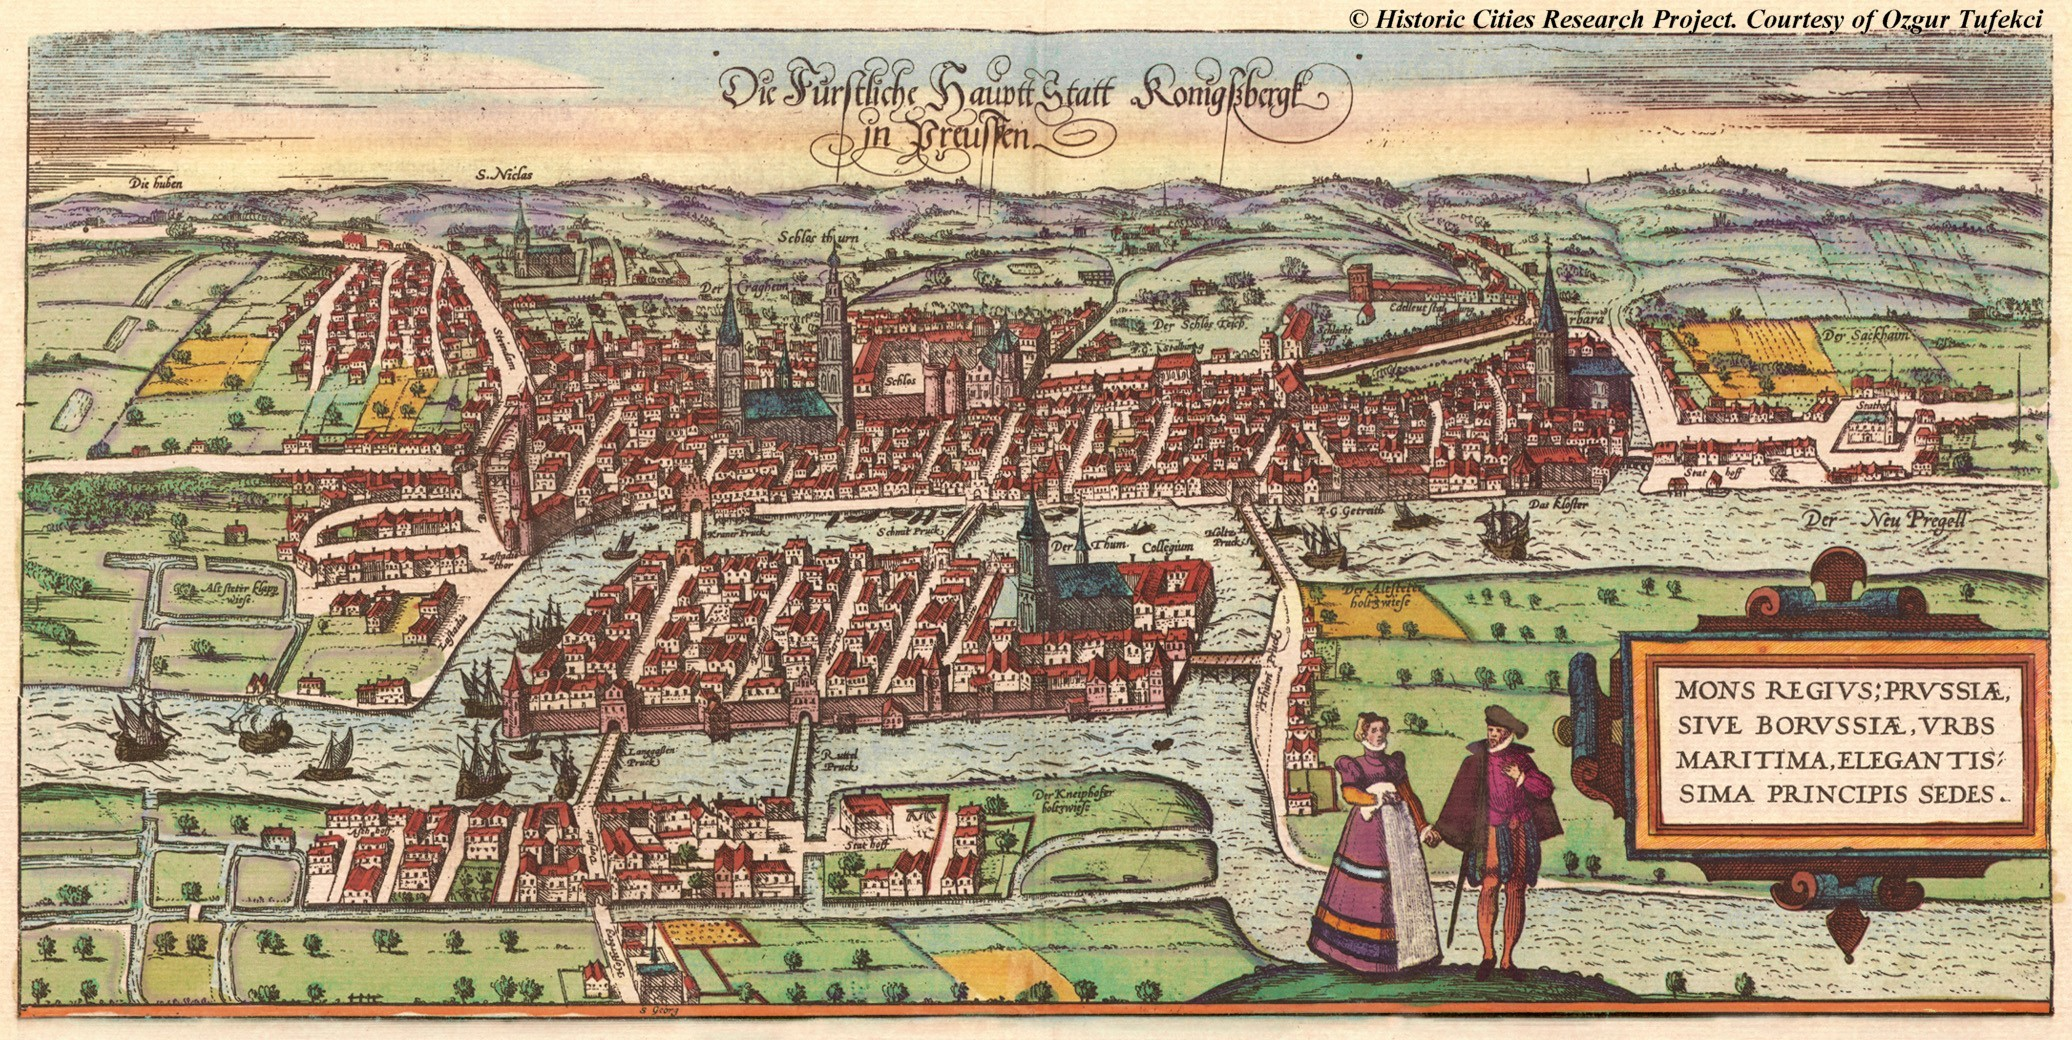
\includegraphics[width=\columnwidth]{../img/konigsberg.jpg}
\\ {\tiny Source: Historical Map / Euler (1736)}
\begin{center}
Seven bridges of Konigsberg.
\end{center}
\end{frame}
%%%%%%%%%%%%%%%%%%%%
\begin{frame}
\frametitle{Graph theory refresher}
\begin{center}
% Manual layout for Königsberg bridges (spring layout needs lualatex)
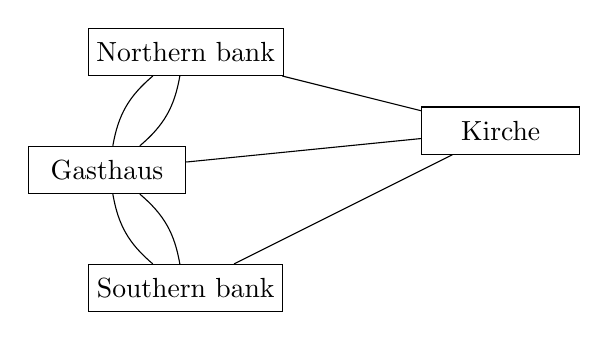
\begin{tikzpicture}[every node/.style={draw, rectangle, minimum width=2cm, minimum height=0.6cm, inner sep=3pt}]
\node (N) at (0,2) {Northern bank};
\node (K) at (4,1) {Kirche};
\node (S) at (0,-1) {Southern bank};
\node (G) at (-1,0.5) {Gasthaus};
\draw (N) -- (K);
\draw (K) -- (S);
\draw (G) -- (K);
\draw[bend left=20] (N) to (G);
\draw[bend right=20] (N) to (G);
\draw[bend left=20] (G) to (S);
\draw[bend right=20] (G) to (S);
\end{tikzpicture}
\end{center}
\end{frame}
%%%%%%%%%%%%%%%%%%%%%%%%%%%%%%%%%%%%%%%%%%%%%%%%%%%%%%%%%%%%%




%%%%%%%%%%%%%%%%%%%%%%%%%%%%%%%%%%%%%%%%%%%%%%%%%%%%%%%

%%%%%%%%%%%%%%%%%%%%





\MakeLastSlide
\end{document}
